\documentclass[oneside,12pt]{book}
%\documentclass[oneside,12pt]{article}
\usepackage{xltxtra,fontspec,xunicode}
\usepackage[slantfont,boldfont]{xeCJK} % 允许斜体和粗体
\usepackage{titlesec}
\usepackage{graphicx}
\usepackage{skull}
\usepackage{fancyhdr}
\usepackage{listings}
\usepackage{xcolor}

\usepackage[ plainpages = false, pdfpagelabels, 
             bookmarks,
             bookmarksopen = true,
             bookmarksnumbered = true,
             breaklinks = true,
             linktocpage,
             pagebackref,
             colorlinks = true,
             linkcolor = blue,
             urlcolor  = blue,
             citecolor = red,
             anchorcolor = green,
             hyperindex = true,
             hyperfigures
             ]{hyperref}
             

\titleformat{\chapter}[display]{\centering\Huge\bfseries}{}{1em}{}
%\setCJKmainfont{SimSun}
%\setCJKmainfont{仿宋}
\setCJKmainfont{微软雅黑}



\usepackage{nomencl}
\makenomenclature
\renewcommand\nomgroup[1]{%
  \ifthenelse{\equal{#1}{A}}{%
   \item[\textbf{Roman Symbols}] }{%             A - Roman
    \ifthenelse{\equal{#1}{G}}{%
     \item[\textbf{Greek Symbols}]}{%             G - Greek
      \ifthenelse{\equal{#1}{R}}{%
        \item[\textbf{Superscripts}]}{%              R - Superscripts
          \ifthenelse{\equal{#1}{S}}{%
           \item[\textbf{Subscripts}]}{{%             S - Subscripts
	    \ifthenelse{\equal{#1}{X}}{%
	     \item[\textbf{Other Symbols}]}{{%    X - Other Symbols
	    \ifthenelse{\equal{#1}{Z}}{%
	     \item[\textbf{Acronyms}]}%              Z - Acronyms
              			{{}}}}}}}}}}
\setlength{\hoffset}{0.00cm}
\setlength{\voffset}{0.00cm}

\setlength{\evensidemargin}{1.96cm}
%\setlength{\oddsidemargin}{-0.54cm}
\setlength{\topmargin}{1mm}
\setlength{\headheight}{1.36cm}
\setlength{\headsep}{1.00cm}
\setlength{\textheight}{20.84cm}
\setlength{\textwidth}{14.5cm}
\setlength{\marginparsep}{1mm}
\setlength{\marginparwidth}{3cm}
\setlength{\footskip}{2.36cm}

%据说可以调整行距
\renewcommand{\baselinestretch}{1.62}
\title{\textit{内核笔记}}
\date{2016-09-09}
\pagestyle{fancy}                    % 设置页眉






\author{\href{mailto:dhacklove@163.com}{段武杰}}

\begin{document}    %文档开始
\maketitle          %插入标题
\setcounter{secnumdepth}{4}
\setcounter{tocdepth}{3}
\renewcommand{\contentsname}{目录}
%\renewcommand\refname{参考文献}
\renewcommand\bibname{参考文献}
%\lhead{我生于贫穷,但不能死于贫穷}

\pdfbookmark[1]{目录}{anchor} %将目录加入标签
\tableofcontents    %插入目录
\mainmatter % book mode only

%\chapter{介绍}

我有一个缺点,对于所有未知的事物我都想去知道,这导致随着我的工作的进行,就变得越来越厌倦工作了,总以为不管努不努力,我都能很好的
完成,这样工作就变得乏味起来,失去了兴趣,但当我开始了解市场时,我就迷上了,因为明天永远是未知的,市长也总是在变化,自己永远不会
有精通的一天,必须不断的适应市场,必须不断的认错,不断的冒险,不断的学习,对我来说这个行当是完美的工作,因为永远有事做,永远在变化!

注重过程而不是利润,当你在注重利润的时候,你就变的一无所有了!


本书想通过技术分析,经济数据分析和反身性理论来发展索罗斯的反身性理论,以期望解决如何作出具体预言的步骤! 

索罗斯在提出反身性的哲学时,对基本面分析和和技术分析都全盘否定,反身性理论也并没有找到好的方式来进行为来作出具体预言!
根据反身性理论在不完备的知识和参与者的偏向情况下,预言和事件一定会存在失真,因此产生了将基本分析和技术分析应用于反身性理论
以让预言和事件无限的接近!并提出一个能大概率进行预言的反身性系统与工具!

基本数据间的反身性,我们认为主流偏向是一个相对的概念,两个国家之间只会存在相对较好和相对较差两种,因此在两国之间
只会存在一个主流偏向,并随着时间的改变进行加强或修正.



\textbf{•}
%\chapter{To-Do}

\begin{itemize}
\item 
\item
\item
\item

\end{itemize}

[credential]
	helper = store
%\chapter{认识自己}


心急是我最大的缺点!


       %认识自己
%\chapter{交易系统胜算}
注意这一定是按照交易系统的开仓次数
\begin{itemize}
\item 开仓次数: 3
\item 亏损次数: 1
\item 盈利次数:
\item 胜率:
\end{itemize}   %交易系统胜算计算
%\chapter{市场认知}
\begin{itemize}
\item 没当有重要经济数据公布时,都会对市场造成重要的波动。
\item 市场的健康程度严重影响,货币波动 .动荡不安的货币价值更低
\item 经济状况及国内稳定的国家,货币趋于稳定!货币价值更高!
\item 各个国家都会按照自己国家利益最大化来对市场做出策略,当自己做出策略时,需要看是否符合国家的利益
\item 在市场动荡不安时,应该选择经济最稳定的国家!作为对象
\item 货币的价格通过供求关系及市场的反身性关系来相互影响和决定的!
\end{itemize}       %市场认知
\chapter{内存寻址}



\paragraph{}
\paragraph{}
\paragraph{}
\paragraph{}
\paragraph{}
\paragraph{}
\paragraph{}
\paragraph{}
\paragraph{}
\paragraph{}











\section{没有高速缓存的转换过程}

在没有高速缓存的情况下虚拟地址的转换过程:

\begin{figure}[htbp]
\begin{center}
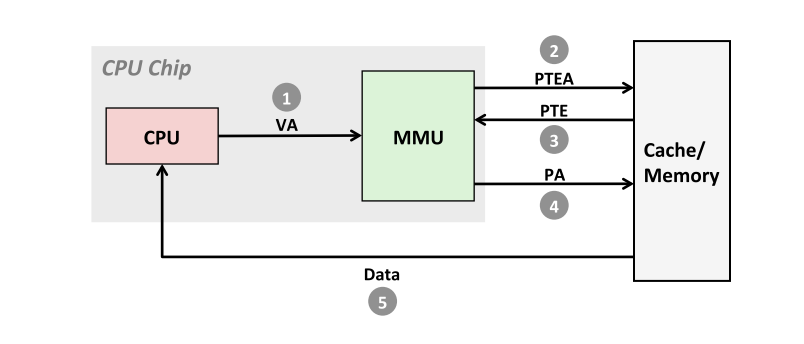
\includegraphics[width=1\textwidth]{slowvava.png}
\caption{没有高速缓存对数据的访问}
\end{center}
\end{figure}

\begin{enumerate}
\item Processor sends virtual address to MMU
\item MMU fetches PTE from page table in memory(Access memory once)
\item MMU sends physical address to memory(Access memory twice)
\item Memory send sdata word to processor	
\end{enumerate}

因此在没有高速缓存的情况下,CPU读取数据会进行2次内存访问,其中1次读取页表,1次读取数据。

\section{有高速缓存的转换过程}


在有高速缓存的情况下虚拟地址的转换过程:


\begin{enumerate}
\item 处理器将虚拟地址发送给MMU
\item MMU根据PTEA从cache中读取pte,如果命中cache则使用转换出的物理地址读取内存数据。
\item 如果没有命中cache,则重内存中取得pte并更新cache,再重内存中读取数据(最多读取2次内存)
\end{enumerate}


\begin{figure}[!htbp]
\begin{center}
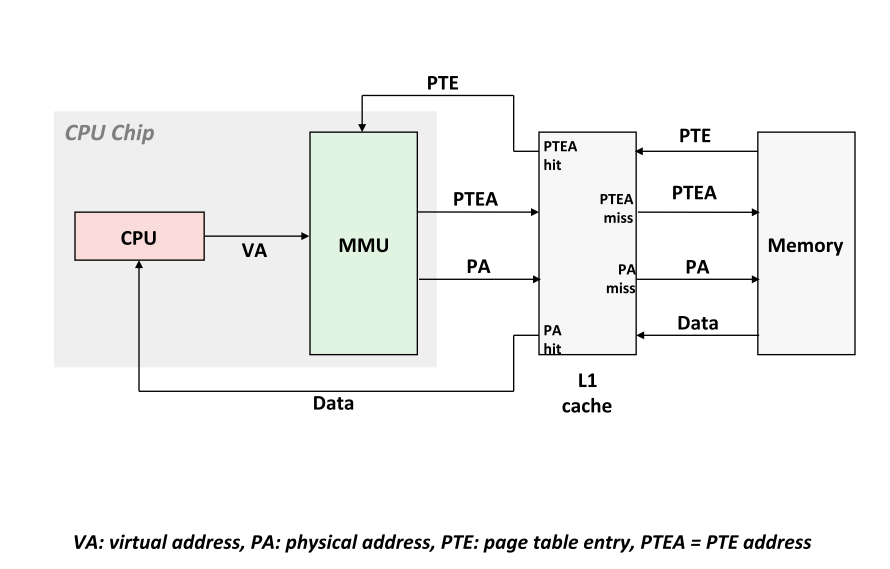
\includegraphics[width=1\textwidth]{highvava.png}
\caption{有高速缓存时对数据的访问}
\end{center}
\end{figure}

由于局部性原理,cache命中的概率很高,这样就减少了对内存的直接访问,从而提高了访问速度。



\section{Linux中的分页}

\paragraph{}

\begin{figure}[!htbp]
\begin{center}
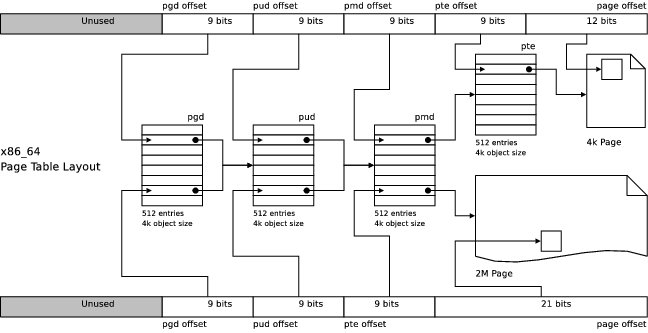
\includegraphics[width=1\textwidth]{va-to-pa.png}
\caption{虚拟地址转换\cite{linuxmm}}
\end{center}
\end{figure}


\begin{itemize}
\item PGD:页全局目录(Page Global Directory)
\item PUD:页上级目录(Page Upper Directory)
\item PMD:页中间目录(Page Middle Directory)
\item PT:页表(Page Table)
\item PTE:页表项(Page table entry)
\end{itemize}

页全局目录包含若干页上级目录的地址,页上级目录包含若干页中间目录的地址,而页中间目录又包含若干页表的地址
。每一个页表项指向一个页框。线程地址被分成5部分。

\section{PTE结构}

Core i7的页表结构:

\begin{figure}[htbp]
\begin{center}
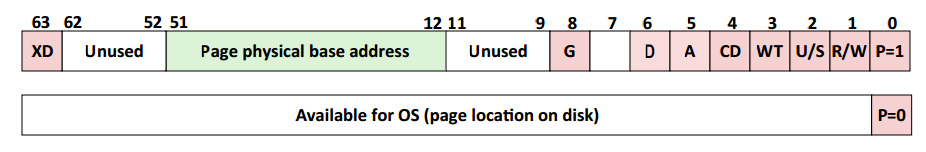
\includegraphics[width=1\textwidth]{pte.png}
\caption{Core i7 Level 4 Page Table	Entries}
\end{center}
\end{figure}


\begin{itemize}
\item \textbf{P:} Child page is present in memory (1)or not(0)	
\item \textbf{R/W:} Read-only or read-write access permission for child page	
\item \textbf{U/S:} User or	supervisor mode	access	
\item \textbf{WT:} Write-through or	write-back cache policy for this page	
\item \textbf{CD:} Cache disabled (1) or	enabled (0)	
\item \textbf{A:} Reference bit (set by MMU on reads and	writes, cleared	by sohware)	
\item \textbf{D:} Dirty bit (set	by MMU on writes, cleared by sohware)	
\item \textbf{G:} Global	page (don’t	evict from TLB on task switch)	
\item \textbf{Page physical base address:} 40 most significant bits of physical page address (forces pages to be	4KB	aligned)	
\end{itemize}



       %交易策略
%\chapter{文件系统}




\section{inode}

内核处理文件的关键是inode,每个文件(和目录)都有且只有一个对应的inode,其中包含元数据(如访问权限,上次
修改的日期,等等)和指向文件数据的指针。

\begin{lstlisting}[language={[ANSI]C},
        basicstyle=\tiny\ttfamily,
        stringstyle=\color{purple},
        keywordstyle=\color{blue}\bfseries,
        commentstyle=\color{olive},
        directivestyle=\color{blue},
        frame=shadowbox,
        %framerule=0pt,
        %backgroundcolor=\color{pink},
        rulesepcolor=\color{red!20!green!20!blue!20}
        %rulesepcolor=\color{brown}
        %xleftmargin=0em,xrightmargin=0em,aboveskip=0em
        ]


/*
 * Keep mostly read-only and often accessed (especially for
 * the RCU path lookup and 'stat' data) fields at the beginning
 * of the 'struct inode'
 */
struct inode {/* fs.h */
	umode_t			i_mode;/* 文件访问权限和所有权 */
	unsigned short		i_opflags;
	kuid_t			i_uid;/* uid about the file */
	kgid_t			i_gid;/* gid about the file */
	unsigned int		i_flags;

#ifdef CONFIG_FS_POSIX_ACL
	struct posix_acl	*i_acl;
	struct posix_acl	*i_default_acl;
#endif
	/* 负责管理结构性操作(如删除一个文件)和文件相关的元数据(例如属性) */
	const struct inode_operations	*i_op;
	struct super_block	*i_sb;
	struct address_space	*i_mapping;

#ifdef CONFIG_SECURITY
	void			*i_security;
#endif

	/* Stat data, not accessed from path walking */
	/* 对给定的文件系统,唯一的编号标识 */
	unsigned long		i_ino;
	/*
	 * Filesystems may only read i_nlink directly.  They shall use the
	 * following functions for modification:
	 *
	 *    (set|clear|inc|drop)_nlink
	 *    inode_(inc|dec)_link_count
	 */
	union {
		/* 记录使用该 inode 的硬链接总数 */
		const unsigned int i_nlink;
		unsigned int __i_nlink;
	};
	dev_t			i_rdev;
	
	loff_t			i_size;/* 文件大小 */
	struct timespec		i_atime;/* 最后访问时间 */
	struct timespec		i_mtime;/* 最后修改时间*/
	struct timespec		i_ctime;/* inode 最后修改时间 */
	spinlock_t		i_lock;	/* i_blocks, i_bytes, maybe i_size */
	unsigned short          i_bytes;
	unsigned int		i_blkbits;
	blkcnt_t		i_blocks;/*指定了按块存放的长度*/

#ifdef __NEED_I_SIZE_ORDERED
	seqcount_t		i_size_seqcount;
#endif

	/* Misc */
	unsigned long		i_state;
	struct mutex		i_mutex;

	unsigned long		dirtied_when;	/* jiffies of first dirtying */
	unsigned long		dirtied_time_when;

	struct hlist_node	i_hash;
	struct list_head	i_io_list;	/* backing dev IO list */
#ifdef CONFIG_CGROUP_WRITEBACK
	struct bdi_writeback	*i_wb;		/* the associated cgroup wb */

	/* foreign inode detection, see wbc_detach_inode() */
	int			i_wb_frn_winner;
	u16			i_wb_frn_avg_time;
	u16			i_wb_frn_history;
#endif
	struct list_head	i_lru;		/* inode LRU list */
	struct list_head	i_sb_list;
	union {
		struct hlist_head	i_dentry;
		struct rcu_head		i_rcu;
	};
	u64			i_version;
	atomic_t		i_count;/* 访问该inode的进程数目 */
	atomic_t		i_dio_count;
	atomic_t		i_writecount;
#ifdef CONFIG_IMA
	atomic_t		i_readcount; /* struct files open RO */
#endif

	const struct file_operations	*i_fop;	/* 用于操作文件中包含的数据 */
	struct file_lock_context	*i_flctx;
	struct address_space	i_data;
	struct list_head	i_devices;
	union {
		struct pipe_inode_info	*i_pipe;
		struct block_device	*i_bdev;
		struct cdev		*i_cdev;
		char			*i_link;
	};

	__u32			i_generation;

#ifdef CONFIG_FSNOTIFY
	__u32			i_fsnotify_mask; /* all events this inode cares about */
	struct hlist_head	i_fsnotify_marks;
#endif

	void			*i_private; /* fs or device private pointer */
};


\end{lstlisting}


\section{inode\_operations}

大多数请况下,各个函数指针成员的意义可以根据其名称推断。它们与对应的系统调用和用户空间工具
在名称方面非常相似。

\begin{lstlisting}[language={[ANSI]C},
        basicstyle=\tiny\ttfamily,
        stringstyle=\color{purple},
        keywordstyle=\color{blue}\bfseries,
        commentstyle=\color{olive},
        directivestyle=\color{blue},
        frame=shadowbox,
        %framerule=0pt,
        %backgroundcolor=\color{pink},
        rulesepcolor=\color{red!20!green!20!blue!20}
        %rulesepcolor=\color{brown}
        %xleftmargin=2em,xrightmargin=2em,aboveskip=0em
        ]
struct inode_operations {
	/* lookup 根据文件系统对象的名称(表示为字符串)查找其 inode 实例*/
	struct dentry * (*lookup) (struct inode *,struct dentry *, unsigned int);
	const char * (*follow_link) (struct dentry *, void **);
	int (*permission) (struct inode *, int);
	struct posix_acl * (*get_acl)(struct inode *, int);

	int (*readlink) (struct dentry *, char __user *,int);
	void (*put_link) (struct inode *, void *);

	int (*create) (struct inode *,struct dentry *, umode_t, bool);
	int (*link) (struct dentry *,struct inode *,struct dentry *);
	int (*unlink) (struct inode *,struct dentry *);
	int (*symlink) (struct inode *,struct dentry *,const char *);
	int (*mkdir) (struct inode *,struct dentry *,umode_t);
	int (*rmdir) (struct inode *,struct dentry *);
	int (*mknod) (struct inode *,struct dentry *,umode_t,dev_t);
	int (*rename) (struct inode *, struct dentry *,
			struct inode *, struct dentry *);
	int (*rename2) (struct inode *, struct dentry *,
			struct inode *, struct dentry *, unsigned int);
	int (*setattr) (struct dentry *, struct iattr *);
	int (*getattr) (struct vfsmount *mnt, struct dentry *, struct kstat *);
	int (*setxattr) (struct dentry *, const char *,const void *,size_t,int);
	ssize_t (*getxattr) (struct dentry *, const char *, void *, size_t);
	ssize_t (*listxattr) (struct dentry *, char *, size_t);
	int (*removexattr) (struct dentry *, const char *);
	int (*fiemap)(struct inode *, struct fiemap_extent_info *, u64 start,
		      u64 len);
	int (*update_time)(struct inode *, struct timespec *, int);
	int (*atomic_open)(struct inode *, struct dentry *,
			   struct file *, unsigned open_flag,
			   umode_t create_mode, int *opened);
	int (*tmpfile) (struct inode *, struct dentry *, umode_t);
	int (*set_acl)(struct inode *, struct posix_acl *, int);

	/* WARNING: probably going away soon, do not use! */
} ____cacheline_aligned;
\end{lstlisting}
%\chapter{中断处理}

中断的本质是一种特殊的电信号,有硬件发向处理器。内核启用中断以前,必须把IDT表的初始化地址装到idtr寄存器 
,并初始化表中的每一项。
%\section{系统启动}




%\chapter{模块实现}


由于insmod调用系统调用init\_module;该系统调用回调模块初始化函数,所以在模块初始化函数中,属于insmod的进程上下文。


\begin{lstlisting}[language={[ANSI]C},
        basicstyle=\tiny\ttfamily,
        stringstyle=\color{purple},
        keywordstyle=\color{blue}\bfseries,
        commentstyle=\color{olive},
        directivestyle=\color{blue},
        frame=shadowbox,
        %framerule=0pt,
        %backgroundcolor=\color{pink},
        rulesepcolor=\color{red!20!green!20!blue!20}
        %rulesepcolor=\color{brown}
        %xleftmargin=2em,xrightmargin=2em,aboveskip=0em
        ]
struct module {
	enum module_state state;/* 模块的内部状态 */

	/* Member of list of modules */
	struct list_head list;/*模块链表 */

	/* Unique handle for this module */
	char name[MODULE_NAME_LEN];/* 模块名 */

	/* Sysfs stuff. */
	struct module_kobject mkobj;
	struct module_attribute *modinfo_attrs;
	const char *version;
	const char *srcversion;
	struct kobject *holders_dir;

	/* Exported symbols */
	const struct kernel_symbol *syms;
	const unsigned long *crcs;
	unsigned int num_syms;

	/* Kernel parameters. */
#ifdef CONFIG_SYSFS
	struct mutex param_lock;
#endif
	struct kernel_param *kp;
	unsigned int num_kp;

	/* GPL-only exported symbols. */
	unsigned int num_gpl_syms;
	const struct kernel_symbol *gpl_syms;
	const unsigned long *gpl_crcs;

#ifdef CONFIG_UNUSED_SYMBOLS
	/* unused exported symbols. */
	const struct kernel_symbol *unused_syms;
	const unsigned long *unused_crcs;
	unsigned int num_unused_syms;

	/* GPL-only, unused exported symbols. */
	unsigned int num_unused_gpl_syms;
	const struct kernel_symbol *unused_gpl_syms;
	const unsigned long *unused_gpl_crcs;
#endif

#ifdef CONFIG_MODULE_SIG
	/* Signature was verified. */
	bool sig_ok;
#endif

	bool async_probe_requested;

	/* symbols that will be GPL-only in the near future. */
	const struct kernel_symbol *gpl_future_syms;
	const unsigned long *gpl_future_crcs;
	unsigned int num_gpl_future_syms;

	/* Exception table */
	unsigned int num_exentries;
	struct exception_table_entry *extable;

	/* Startup function. */
	int (*init)(void);

	/*
	 * If this is non-NULL, vfree() after init() returns.
	 *
	 * Cacheline align here, such that:
	 *   module_init, module_core, init_size, core_size,
	 *   init_text_size, core_text_size and mtn_core::{mod,node[0]}
	 * are on the same cacheline.
	 */
	void *module_init	____cacheline_aligned;

	/* Here is the actual code + data, vfree'd on unload. */
	void *module_core;

	/* Here are the sizes of the init and core sections */
	unsigned int init_size, core_size;

	/* The size of the executable code in each section.  */
	unsigned int init_text_size, core_text_size;

#ifdef CONFIG_MODULES_TREE_LOOKUP
	/*
	 * We want mtn_core::{mod,node[0]} to be in the same cacheline as the
	 * above entries such that a regular lookup will only touch one
	 * cacheline.
	 */
	struct mod_tree_node	mtn_core;
	struct mod_tree_node	mtn_init;
#endif

	/* Size of RO sections of the module (text+rodata) */
	unsigned int init_ro_size, core_ro_size;

	/* Arch-specific module values */
	struct mod_arch_specific arch;

	unsigned int taints;	/* same bits as kernel:tainted */

#ifdef CONFIG_GENERIC_BUG
	/* Support for BUG */
	unsigned num_bugs;
	struct list_head bug_list;
	struct bug_entry *bug_table;
#endif

#ifdef CONFIG_KALLSYMS
	/*
	 * We keep the symbol and string tables for kallsyms.
	 * The core_* fields below are temporary, loader-only (they
	 * could really be discarded after module init).
	 */
	Elf_Sym *symtab, *core_symtab;
	unsigned int num_symtab, core_num_syms;
	char *strtab, *core_strtab;

	/* Section attributes */
	struct module_sect_attrs *sect_attrs;

	/* Notes attributes */
	struct module_notes_attrs *notes_attrs;
#endif

	/* The command line arguments (may be mangled).  People like
	   keeping pointers to this stuff */
	char *args;

#ifdef CONFIG_SMP
	/* Per-cpu data. */
	void __percpu *percpu;
	unsigned int percpu_size;
#endif

#ifdef CONFIG_TRACEPOINTS
	unsigned int num_tracepoints;
	struct tracepoint * const *tracepoints_ptrs;
#endif
#ifdef HAVE_JUMP_LABEL
	struct jump_entry *jump_entries;
	unsigned int num_jump_entries;
#endif
#ifdef CONFIG_TRACING
	unsigned int num_trace_bprintk_fmt;
	const char **trace_bprintk_fmt_start;
#endif
#ifdef CONFIG_EVENT_TRACING
	struct trace_event_call **trace_events;
	unsigned int num_trace_events;
	struct trace_enum_map **trace_enums;
	unsigned int num_trace_enums;
#endif
#ifdef CONFIG_FTRACE_MCOUNT_RECORD
	unsigned int num_ftrace_callsites;
	unsigned long *ftrace_callsites;
#endif

#ifdef CONFIG_LIVEPATCH
	bool klp_alive;
#endif

#ifdef CONFIG_MODULE_UNLOAD
	/* What modules depend on me? */
	struct list_head source_list;
	/* What modules do I depend on? */
	struct list_head target_list;

	/* Destruction function. */
	void (*exit)(void);

	atomic_t refcnt;
#endif

#ifdef CONFIG_CONSTRUCTORS
	/* Constructor functions. */
	ctor_fn_t *ctors;
	unsigned int num_ctors;
#endif
} ____cacheline_aligned;

\end{lstlisting}

%\include{内核数据结构}
%\chapter{模板}

\begin{lstlisting}[language={[ANSI]C},
        numbers=left,
        numberstyle=\tiny,
        basicstyle=\small\ttfamily,
        stringstyle=\color{purple},
        keywordstyle=\color{blue}\bfseries,
        commentstyle=\color{olive},
        directivestyle=\color{blue},
        frame=shadowbox,
        %framerule=0pt,
        %backgroundcolor=\color{pink},
        rulesepcolor=\color{red!20!green!20!blue!20}
        %rulesepcolor=\color{brown}
        %xleftmargin=2em,xrightmargin=2em,aboveskip=1em
        ]
int main(int argc, char ** argv)
{
	printf("Hello world!\n");
	return 0;
}
\end{lstlisting}
%\chapter{经济数据分析}

\section{CRB指数}

反映的是美国商品价格的总体波动,能使机构和个人投资者利用指数交易而获得商品价格综合变动带来的获利机会。


在分析数据时应当从数据本身进行分析,即从原数据分析,不能使用别人消化过后的观点!

汇率是由外汇的供求关系决定的,以下是影响汇率的主要因素:
\begin{itemize}
\item 利率
\item 经济活动水平
\item 非投机资本流
\item 投机资本流
\item 贸易平衡
\item 政府预算
\item 地缘政治事件
\end{itemize}

\section{利率}

\begin{itemize}
\item \textbf{存款利率(Deposit interest rate)}: 个人或企业将钱存入银行,银行所需付出的货币价格!
\item \textbf{借款利率(Lending interest rate )}:银行将钱借给个人或企业,个人或企业所需付出的货币价格!
\item \textbf{真实利率(Real interest rate)}:去除通货膨胀后的利率。
\end{itemize}

\section{经济活动水平}
\section{非投机资本流}
\section{投机资本流}
\section{贸易平衡}
\section{政府预算}


\section{美国经济数据分析}



\subsection{利率}



贷款利率从08年金融危机以来从5.1跌至3.3并连续4年内保持在3.3,降低借款利率的原因是美联储想

\href{http://data.worldbank.org/indicator/FR.INR.RINR/countries/US?display=graph}{美国真实利率},从2011年到现在来看,美国的真实利率在逐步增加,这样今天调高利率的可能性也可能会增大



\subsection{通货膨胀率}

通货膨胀的相关数据一般反应了总体物价水平的上升速度。通货膨胀会造成购买力下降,所以调控通货膨胀非常重要。通常来说通胀率上升标志着该经济发展的过快,而通胀率下降标志着经济急剧萎缩。

\begin{itemize}
\item 消费者物价指数(CPI)
\item 通货膨胀率计算公式
\end{itemize}
$$Inflation Rate=\frac{Current CPI-Base CPI}{Base CPI}*100\%$$

\subsection{就业率}
在一个经济体中就业率越高说明经济状况越良好这个指标和利率一样是个关键指标
\begin{itemize}
\item 非农就业人口,上个月新增的非农就业机会
\item 失业率:正在积极寻找工作而尚未获得工作职位的人所占的比例
\end{itemize}

就业人口从2008年的负值,就业人数开始逐步增加,这两年每个月的非农就业人口趋于稳定,说明美国经济在往好的方面发展!

失业率:从2008年~2009年增加,从2011年~2015年开始减少,说明美国经济在往好的方面发展!

\subsection{GDP国内生产总值}
\href{http://data.worldbank.org/indicator/NY.GDP.MKTP.KD.ZG/countries/1W-US?display=graph}{GDP}


GDP是在某一既定时期一个国家内生产的所有最终物品与劳务的市场价值,美国的GDP增长率是相对于2005年的GDP来说的!


经济增长的相关数据显示了经济体的经济发展程度,国家经济通常有3个发展方向:一是发展,二是停滞,三是收缩,经济体在不断发展时,该经济的各个方面都运作良好,并实现盈利性增长。如果经济体总是处于停滞或者收缩状态,其货币会遭受打击,走势疲软!疲软你懂的!

经济增长的的情况主要表现在国内生产总值中!


\subsection{国际贸易收支}

\subsection{海外投资}
\subsection{消费信心}



\section{加拿大经济数据分析}

\href{http://data.worldbank.org/indicator/FR.INR.RINR/countries/CA?display=graph}{加拿大真实利率}

\section{欧盟区经济数据分析}


\section{澳大利亚数据分析}
    %经济数据分析
%\chapter{技术分析}

最後再次告诫投资者∶不要盲目跟风,不要做趋势尾部的“博傻者”,如果你真的希望押注欧元长期趋势向下,请耐心等待汇价充分修正後再进场,否则可能陷入过度贪婪的陷阱。

合适的入场价格很重要!

\section{布林带}
\begin{itemize}

\item 用来衡量市场的波动。
\item 他们的行为就像是迷你的支持和阻力水平。
\item 布林线反弹:一个策略上的概念,价格往往总是回到布林线中间地带。
\item 布林线挤压:当布林线挤压时,意味着市场是非常安静的,需要一个杰出的突破。 一旦爆发,无论在什么方面,当我们进入交易时都是在寻求突破。
\end{itemize}


\section{RSI}

\section{MACD}

\section{多重时间段分析}


多重时间段分析是透过观察相同货币对多个不同时间段图表而分析货币对的方法。其优点是藉观察较长的时间段,然后再看较短的时间段,继而再看更短的时间段,交易者将可对货币对如何移动有更详细的了解,从而在更有根据的情况下建立交易。


一般而言,交易者会选择三个时间段,而有关时间段将会根据交易者的个人交易策略而定。较长线交易者可以选择每周、每日及4小时图。较短线交易者可以选择4小时、1小时及15分钟图。重点是以当中最长线的图表来厘定“整体趋势”及应朝哪一个方向买卖。其后使用较短的时间段来“微调”在该个方向哪一个水平建立持仓。


您可能曾经听说过“趋势中存在趋势”。例如,在日图中,趋势可能是一个升势,而在4小时图中,则可能是跌势,在1小时图中可能是持平… 所有趋势都是关于同一个货币对。

在此情景下,整体趋势以日图为基础 – 即上升。然而,在这个升势之内,于4小时的时间段内则出现转势。转势很可能在某一点结束,而4小时时间段则与日图趋于一致。同样道理,在4小时时间段内存在1小时的趋势。随着1小时趋势与4小时趋于一致,而4小时与日图趋于一致,一个有机会更高的入市点将会出现。

总括来说,当最短的时间段完成转势(转势指我们在日图中注意到与趋势相反的走势),及开始重新朝每日趋势的方向移动时,我们便希望建立交易。这就是我们的入市信号。

试想像它们是一个密码锁的制栓,全部都有次序地趋于一致。

透过使用数个时间段,交易者可以在三个不同层面上深入了解货币对,及学习运用该些资料,以成功地在时间段所示成功机率最高的时候建立交易。


%\section{反身性尝试}

\begin{itemize}
\item 如何判断一个国家的经济好坏!

\end{itemize}
%\section{Pro to do}

\begin{itemize}
\item 每天保持整洁
\item 考上驾照
\item 我生于贫穷,但不能死于贫穷!
\item 穷,是说你口袋里面有多少和你心里面有多少。
\item 人的一切痛苦,本质上都是对自己的无能的愤怒!
\item 做个更好的人!
\item 床是哪来睡觉的人!

\item 索罗斯有一个良好的生活习惯!
\item 索罗斯很懂经济学,金融学,银行学


\item 先做模拟外汇,等能够稳定盈利了再,实盘

\item 让自己的资金滚动起来

\item 招行账单日是每月3号,如果要达到最长免息就得在账单日后1天消费,也就是每月的4号,这样到下个月的21号还款!
\item  

\end{itemize}



%\section{交易日志}



\subsection{2015-01-16}
\begin{itemize}
\item 从经济数据上今天晚上公布美国12月核心消费者物价指数年率,如果高于预期,这将提振美元。
\item 从技术分析上看,USDCAD日图和周图均线仍呈多头排列,显示趋势的强劲。
\item 相对强度分析:AUDCAD 澳元强于加元,NYDCAD 纽元强于加元,
\item 潜在风险:美国消费物价指数低于预期,将会引起一定USDCAD一定的震荡!
\item 短期趋势:高位震荡
\item 因此从经济数据和技术分析看,今天可以在RSI接近超卖的低位进入做多,轻仓进入
\item 开仓时间:2015-01-16 01:50
\item 开仓部位:0.11手
\item 止损:1000,止盈:5000,可能亏损金额:100\$,策略完成可能赚取的金额:500
\item 理论风险回报比 5:1
\item 实际风险回报比
\item 平仓时间:
\item \textcolor{red}{亏损原因:在识别出图形模式后,没有及时将反向单平仓!而且在不合适的时机作出了对冲的操作!}
\item 这是一个失败的交易:在没有分析出趋势的情况下进行了买入,而且不是在很好的买点买入的!
\end{itemize}
	       %交易日志
%\section{黑客}

\subsection{两头做}





\subsection{大师足迹}


\subsubsection{保罗·都铎·琼斯}

1987年10月,世界上大部分投资者损失惨重。同一个月,保罗•都铎•琼斯掌管的都铎基金却获得62\%的收益。琼斯的出色表现是一贯的,他曾经连续5年保持三位数的增长,1992年底欧洲货币体系发生危机,琼斯数月内在外汇市场赢利十几亿美元。琼斯从做经纪人起家,1976年开始做起,第二年就赚了100多万美元佣金。1980年琼斯到纽约棉花交易所当现场交易员,几年之内赚了上千万。1984年琼斯离开交易所,创建都铎基金,从150万做起。4年后投资到他的基金的每1000美元已增值到1700多美元。到1992年底,都铎基金总额已增长到60亿美元。如果不是琼斯于1987年底停止接受新投资并开始分发利润,那么60亿是绝对打不住的。


琼斯的交易生涯并非一帆风顺。1979年他逞一时之勇,一次进单过多,结果连遇跌停板,等平单出场时资金损失达三分之二。他懊丧至极,对自己几乎完全丧失信心,差一点改行。\textbf{从那以后他开始学会控制风险,遵守原则。}


\textbf{琼斯做单每天都是新的起点,昨天赚的成为过去,今天从零开始。每个月亏损最多不能超过10\%。}顺手时,琼斯可以连续十几个月不输钱。三位数的年增长率对他来说是司空见惯。由于风险控制得法,琼斯的基金在分析判断失误的情况下仍能赢利。1992年年初,琼斯认为美国减息己到尽头,欧洲利息将下降,欧美利率差的缩小将扭转美元弱势。都铎基金因而进场买了大量美元。刚开始还较顺利,美元果然走强了几百点。但不久美国经济不振的消息频传,美元对欧洲货币大幅下跌,直至创历史最低价位。琼斯在发觉大势不对后及时砍单出场,避免了更大的损失。他同时耐心等待时机,追回损失。年底欧洲货币体系发生危机,英镑、意大利里拉等货币大跌,琼斯及时进场抛售外币,一月之内赚了数亿美元。

琼斯有一些具体的做单原则:\textit{不平均加单。一批单子进场后,市场反走说明判断可能有问题,盲目加单平均价位虽然稍好,但如果方问错了,新加的单只是错上加错。反过来讲,如果你相信方问没错,只是价位不够好,那就不必过于计较。琼斯认为,哪里进单不重要,关键是这一天你是看涨还是看跌}。新手最爱问琼斯:你是买还是卖呀? 琼斯认为他是买还是卖不应该影响旁人对市场的判断。新手也要独立思考。再一个问题就是:你从哪里开始买的? 琼斯认为这也与当天是赚还是赔无关,关键是判断涨与跌。

\textbf{琼斯认为,做单最重要的是防守而不是进攻。他每天都假设自己进的每一张单都是错的,事先设好止蚀位,这样他对最多一次会赔多少心里有数}。琼斯奉劝所有交易员不要逞强,更不能自负。要不停地怀疑你自己,怀疑你的能力,永远不要自以为了不起。\textcolor{red}{一飘飘然就完蛋}。这并不是说对自己毫无信心,信心一定要有,但适可而止。琼斯自言他对这行是越干越怕,因为他知道要保持成绩有多难。\textbf{每次大输往往都是在连续做了些漂亮单后自我感觉良好之际。}

琼斯的做单策略与众不同。他不愿意随大流,很少追势,总喜欢在转势之际赚钱。他自为最大的机会主义者。一旦他发现这种机会,便进场兜底或抛顶。错了马上就砍单,然后再试,往往是试了几次以后开始赚大钱。市场上很多人认为一味找底或顶很危险,要赚钱最好抓势的中段。琼斯十多年来却成功地抓住了不少顶和底。琼斯的理论是,跟势的人要在中段赚钱,止蚀单就得设得很远,一旦被迫砍单,损失就很大。再说市场只有15\%情况下才有势,其他时间都是横走。所以他比较喜欢做两头。

琼斯觉得外汇市场任何人都操纵不了。一般人有种错觉,以为华尔街大户能控制市场价格的变化。琼斯说,他可以进场闹腾一、两天,甚至一个星期,特别是如果时机正确,他进场后加加油,可能造成某种假象,但他一停买,市场价格就会掉下来,除非市场本身就很强劲。他打了个生动的比方:你可以在冰天雪地的阿拉斯加开一家最漂亮的夏装店,但没人买,你总归要破产。琼斯还注意听取同行的意见,特别是战绩较佳的同行。\textcolor{red}{如果自己意见和他们一致,他就多做一点,如果有很大分歧。他就观望。本来他看好某一种货币想买进,但得知某位高手在抛出时,他就耐心等待}.到有一天市场开始走平,那人说;我看该出场了,他就进场大买特买。琼斯在具体分析手段方面最推崇"艾略特波"理论。他认为自己的成功很大一部分应归功于这一周期理论。\textbf{艾略特波理论是凭借黄金分割法推算市场涨跌周期的一种分析方法},在股票和期货市场广为采用。琼斯认为外汇市场也不例外。艾略特波理论吃透后,可以帮你找到很多低风险高收益的进单机会。`


谈到成功的秘诀,琼斯认为自己的长处是超脱。\textbf{任何已经发生的事都成为过去,3秒钟之前发生的事无关紧要},关键是下一步怎么办。感情上离市场要远一点,以前的看法不对就得及时修改。思想要开放,信心要坚定。他自己虽然偏好做两头,找逆转,但都锋基金也采用了几套跟势的电脑交易系统,成绩也很不错。但琼斯认为好交易员应该比电脑系统能赚钱,因为人脑能够灵活变通,更快地适应市场的变化,以及不同市场之间的差异。


\subsubsection{外汇大师成功经验总结}
\begin{itemize}
\item 大部分炒家都是从场内交易员开始入行的,随着交易规模啝交易品种的增加逐渐走到场外,冠军炒手马丁舒华兹、鹤立鸡群的理查丹尼斯啝超人斯坦利等人虽然开始都有一段适应过程,但他们都很快踏上了成功之路。
\item 风险控制:这是每个大师操盘经验的重中之重。在期货市场上长期生存的关键就是保留资金实力,给自己留下机会,幸免在一两次交易中就耗光实力。每位大师的风险操纵原则不尽相同,有些是以技术图表为依据,大部分是以资金百分比为依据,而笔者最为认同的则是高富拿设止损位的独特方法:\textbf{止损位永远设在图表上重要的价位之外},宁可减少交易量去迁就一个安全的止损位。“炒外汇”另外,风险控制大师海特提出的回避风险原则也值得我们学习,他认为,\textbf{应幸免参与行情过于激烈的品种};当出现大的亏损时要立刻通知客户,减轻心理负担;当出现风险时,要在第一时间砍仓。选择一个行业股票时,要选两家,但不是随便找两家,应选一家最好和一家最差的!
\item 短线和长线:从大部分炒家成功的经历看,他们都有从短线向长线转变的过程。短线对于投机者来说,在分析、记忆力、反应力、心理、交易通道等方面的要求都比较高,就像乒乓球员面对快速扣球只能下意识反应,而没有时间思考,这些需要平时高强度的训练,但大部分投资者湜很少有工夫去训练的,这也是短线投资者亏损面较大的原因之一。超人斯坦利是最为经典的长线炒家,为了幸免在价格波动时自己惊慌平仓出场,不惜远离市场,持仓数月卙臸数年。
\item 成功啝天才:期货市场不存在天才,理查丹尼斯啝维克多斯柏认为,智力、学历有时会成为成功交易的障碍,切勿死要面子、勇于认错、遵守可行的交易规则啝交易系统、善于总结经验,才是成功的关键。
\item 成功的时间:绝大多数大师都是从失败开始的,短则数月,长则十年,重要的是要有坚定的信心並不断总结经验。正所谓:“学者无先,达者为师”。
\item 电脑交易系统:多位大师都提到在交易中很依赖自己设计的电脑交易系统,电脑交易系统可以幸免人为的情绪影响,特别是在市场较为混乱时,还能坚决执行既定的交易计划,使投资者保持前后一致的获胜概率。当然,每个人必须学会开发适合自己的电脑交易系统。
\item 技术分析和内幕消息:多数大师都以技术分析为入市依据,技术分析能给投资者提供准确的入市时机,这是基本面分析法不能实现的。如超人斯坦利在1974年5月买入了小麦期货合约,半年后就翻了50\%,当记者寻问他是否知道俄罗斯购买小麦的内幕消息时,斯坦利回答:“我一点都不知道俄罗斯在买小麦,但图表告诉我有人在买。”大部分投资者无法靠技术分析法获利的原因在于,他们並没有掌握技术分析法的真谛。而作为大户必须同时使用基本分析法,因为他们资金庞大,建立头寸啝离场时间较长,靠技术分析法建立头寸和离场是较为困难的。
\item 人生哲学:期货市场是遵守零啝定律的,个别人赚大钱就意味着大部分人在亏钱。因此,大师的性格是有异于常人的,他们大多孤僻而充满自信,不喜欢和别人谈论行情和消息,习惯于独立分析市场。
\end{itemize}



%\chapter{市场哲学}


所有理论,技术分析,基本分析,终极问题都是想得到市场的运作方式,以及如何精确的预测未来的走势!

\begin{itemize}
\item 反身性
\item 经济学理论


\end{itemize}


%\bibliographystyle{apalike-refs}
%\bibliography{bib.bib}







\bibliographystyle{ieeetr} 
\bibliography{myreference} 




\end{document}
